\section{ePape - Effective Sound Speed Pad\'e Parabolic Equation Code}
\label{sec: ePape}

{\bf ePape} implements a "Parabolic Equation" (PE)\cite{collins2019parabolic} one-way algorithm, originally developed for ocean acoustic applications, with the influence of the winds approximated using the effective sound speed approximation. As such, propagation is restricted to a single range/altitude plane specified by an azimuth. The influence of cross winds is not modeled. The functions of differential operators that arise are approximated using a Pad\'e expansion whose order can be specified. The differential operators are discretized using a finite difference scheme. The Pad\'e approximation provides numerical accuracy at high elevation angles; however, this can not be considered a high angle PE because the effective sound speed approximation limits the elevation angle, as well as the allowable wind speeds. Attenuation by the atmosphere is implemented via the addition of an imaginary part to the wave number. Both stratified and range dependent atmospheres are supported. Ground impedance boundary conditions are also supported; however, no impedance models have been included yet. Propagation over ground topography is not supported in this release.

\subsection{Mathematical Background}
The PE algorithms operate in the frequency domain and are thus approximate solutions to the convective Helmholtz equation. It's natural to work in cylindrical coordinates range $r$, azimuth $\theta$, and altitude $z$. {\bf ePape} uses the effective sound speed approximation\cite{waxler2019propagation} in which the thermodynamic sound speed, $c$, is replace by $c_{\text{eff}}(\theta,z)=c(z)+u(\theta,z)$, where $u$ is the horizontal component of the wind along a given azimuth $\theta$. In this approximation the influence of cross winds is not modeled, causing the propagation to be restricted to a single range/altitude plane, an $r-z$ plane. The plane is fixed by setting an azimuth, $\theta$. In the effective sound speed approximation, the solution depends on azimuth only through the effective sound speed. Similarly, the locally stratified approximation is used, in which $c$ and $u$ can depend on range $r$, but the $r$ dependence is very slowly varying on the scale of acoustic wavelengths so that changes in $c$ and $u$ can be treated by using the value of $c_{\text{eff}}$ at the range step being considered, ignoring the $r$ dependence, which is to say derivatives with respect to $r$, of $c_{\text{eff}}$ at each range step. 


Introduce the effective wave number (we will drop the explicit dependence on azimuth) 
\[
k(z)=\frac{\omega}{c_{\text{eff}}(z)}.
\]
If $P(r,z)$ is the acoustic pressure, then 
\begin{equation}\label{eq:eff_snd_helmholtz}
\Big(
\frac{\partial^2}{\partial r^2}+\frac{1}{r}\frac{\partial}{\partial r}
+
\rho_0(z)\frac{\partial}{\partial z}\frac{1}{\rho_0(z)}\frac{\partial}{\partial z}
+
k(z)^2
\Big)P(r,z)=0
\end{equation}
where $\rho_0$ is the mean atmospheric density. The acoustic pressure $P$ is scaled by both the $r^{-\frac{1}{2}}$ geometrical spreading factor and the $\sqrt{\rho_0}$ density factor, 
\begin{equation}\label{eq:scaled_P}
P(r,z)=\sqrt{\frac{\rho_0(z)}{r}}\tilde P(r,z).
\end{equation}
Let $k_0$ be a reference wave number, typically the wave number on the ground, and introduce the far field altitude operator 
\[
Q=\frac{1}{k_0^2}\Big(\frac{d^2}{d z^2}+\tilde k(z)^2-k_0^2\Big),
\]
with 
\begin{equation}\label{eq:wavenumber}
\tilde k(z)
=
\sqrt{k(z)^2-\frac{3}{4}\big(\frac{\rho_0^\prime(z)}{\rho_0(z)}\big)^2
+
\frac{1}{2}\frac{\rho_0^{\prime\prime}(z)}{\rho_0(z)}}.
\end{equation}
Then, in the far field, ignoring terms of order $\frac{1}{r^2}$, 
\begin{equation}\label{eq:eff_snd_range_scaled}
\Big(\frac{\partial^2}{\partial r^2}+k_0^2(1+Q)\Big)\tilde P(r,z)=0.
\end{equation}
Formally factoring the differential operator
\[
\frac{\partial^2}{\partial r^2}+k_0^2(1+Q)
=
\Big(\frac{\partial}{\partial r}+ik_0\sqrt{1+Q}\Big)\Big(\frac{\partial}{\partial r}-ik_0\sqrt{1+Q}\Big)
\]
we see that solutions of 
\[
\Big(\frac{\partial}{\partial r}\pm ik_0\sqrt{1+Q}\Big) \tilde P(r,z)=0
\]
are one way solutions of Eq.\,\ref{eq:eff_snd_range_scaled} in the sense that they represent waves traveling in a single direction, ie. outward in the $-$ case and inward in the $+$ case. We will restrict to the outward going case. 

Dividing out a carrier wave as well,
\[
P =\frac{1}{\sqrt{r}} \tilde P =\frac{e^{ik_0r}}{\sqrt{r}} p,
\]
one finds that 
\begin{equation}\label{eq:parabolic}
\frac{\partial p}{\partial r}=ik_0\big(\sqrt{1+Q}-1\big)p. 
\end{equation}
Here $p$ is thought of as a vector valued function of $r$ indexed by the altitude $z$. Note that Eq.\,\ref{eq:parabolic} is the origin of the name ``Parabolic Equation Method''. In the earliest application of this approach $\sqrt{1+Q}-1$ was approximated by $\frac{\partial ^2}{\partial z^2}$, resulting in a parabolic equation. 

Eq. \ref{eq:parabolic} has a formal solution, 
\[
p(r)=e^{ik_0(\sqrt{1+Q}-1)(r-r_0)} p(r_0)
\]
where $r_0<r$. One thinks of $p(r)$ as having been propagated out in range from $r_0$ to $r$. The PE algorithm is based on the formula (Trotter product formula \cite{stoer2013introduction} 
\begin{equation}\label{eq:trotter_prod}
p(r)=\lim_{N\rightarrow\infty}\Big(e^{ik_0(\sqrt{1+Q}-1)\frac{r-r_0}{N}}\Big)^N p(r_0)
\end{equation}
so that letting 
\[
\Delta r=\frac{r-r_0}{N}
\]
and q

\[
r_j=r_0+j\Delta r
\]
one has the approximation 
\begin{equation}\label{eq:split_step}
p(r_j)=e^{i\delta(\sqrt{1+Q}-1)}p(r_{j-1})
\end{equation}
with $\delta=k_0\Delta r$. This allows us to march out from $r_0$ to $r$ if an efficient approximation for $e^{i\delta(\sqrt{1+Q}-1)}$ can be found. The atmospheric profile can be changed as required. Generally, $r_0$ is some small reference range and the starting pressure field, $p_0=p(r_0)$, is called the starter. The starter is usually chosen in such a way as to mimic the signal at range $r_0$ from a point source. In this release, a point source started has been implemented. 

At high enough frequencies the ground can be treated as an impedance plane. This approximation ignores any signal propagation in the substrata and is implemented by imposing the boundary condition 
\begin{equation}\label{eq:impedance}
\frac{\partial P(r,z)}{\partial z}\big|_{z=0}=-\frac{i\omega\rho_0(0)}{Z(\omega)}P(r,0)
\end{equation}
where $Z(\omega)$ is the effective ground impedance. This boundary condition influences the operator $Q$. Note that the density scaling effects the boundary condition. One finds that 
\[
\frac{\partial \tilde P(r,z)}{\partial z}\big|_{z=0}
=
-\Big(\frac{i\omega\rho_0(0)}{Z(\omega)}+\frac{\rho_0^\prime(0)}{2\rho_0(0)}\Big)P(r,0).
\]
The additional density dependent terms provide the Lamb wave but are of the same order as the additional density dependent terms in $\tilde k$ and are usually ignored for frequencies above about 0.08 Hz where buoyancy is not significant. 

The ground impedance is to be considered user input, similarly to the atmospheric profiles. It is generally a complex number. As $Z(\omega)\rightarrow \infty$ this becomes the rigid ground condition. This is expected as $\omega\rightarrow 0$. In common practice the ground impedance is set to zero for purposes of infrasound modeling, however, the low frequency behavior of the ground interaction is not well understood. 

To implement Eq.\ref{eq:split_step}, regardless of $Q$, an effective approximation must be found for the action of the operator 
\begin{equation}\label{eq:propagator}
{\cal F}(\delta,Q)=e^{i\delta(\sqrt{1+Q}-1)}
\end{equation}
on functions of altitude. To this end a Pad\'e approximant will be used. The Pad\'e approximant is a best fit rational function of a given order. To approximate ${\cal F}(\delta,x)$, one defines 
\begin{equation}\label{eq:pade}
R(x)=\frac{a_0+a_1x+a_2x^2+\dots+a_nx^n}{1+b_1x+b_2x^2+\dots+b_mx^m}
\end{equation}
and then chooses the coefficients $a_j$ and $b_k$ so that the Taylor expansions of $R$ and ${\cal F}$ coincide up to order $N=n+m$. Explicitly, 
\[
\frac{d^j R}{dx^j}\big|_{x=0}=\frac{d^j {\cal F}}{dx^j}\big|_{x=0}
\]
for $j=0,1,\dots,N$. That gives $N+1$ equations for as many unknown coefficients. If one restricts $m\ge n$ then $R(x)$ remains bounded for large $x$. One then approximates 
\[
{\cal F}(\delta,x)\approx R(x). 
\]
Approximation by a rational function is preferable to approximation by a polynomial, {\it ie} by a Taylor expansion, because polynomials always increase without bound for large argument. If we insist, as we will, that $m\ge n$ then the approximating function, $R(x)$, is bounded. 

To determine the coefficients $a_j$ and $b_j$ we will need the Taylor coefficients, $c_j$, of ${\cal F}$, 
\[
{\cal F}(\delta,\xi)=\sum_{n=0}^\infty c_n(\delta) \xi^n
\]
Thompson\cite{roberts2013numerically} has derived a recursion relation for the expansion coefficients $c_n$, 
\[
c_{n+1}=-\frac{2n-1}{2(n+1)}c_n-\frac{\delta^2}{4n(n+1)}c_{n-1}. 
\]
This makes the computation of the expansion coefficients very efficient. Note that $c_0=1$ and $c_1=i\frac{\delta}{2}$. Then the $a_j$ and $b_j$ are determined by the condition that that the Taylor expansion of the function 
\[
{\cal F}(\delta,x)-R(x)
=
\sum_{j=0}^\infty c_j(\delta) x^j-\frac{\sum_{l=0}^n a_lx^l}{1+\sum_{k=1}^m b_kx^k}
\]
begin at order $x^{m+n+1}$. This is equivalent to the coefficients in the power series 
\[
\big(\sum_{j=0}^\infty c_j(\delta) x^j\big)\big(1+\sum_{k=1}^m b_kx^k\big)
-
\sum_{l=0}^n a_lx^l
\]
be zero for powers less than or equal to $m+n$. This recursion leads to a sequence of equations. At index $0$,  
\[
a_0=c_0,
\]
for $i=1,2,\dots,n$, 
\[
\sum_{j=0}^{i-1}c_jb_{i-j}-a_i=-c_i, 
\]
for $i=n+1,n+2,\dots,m$, 
\[
\sum_{j=0}^{i-1}c_jb_{i-j}=-c_i,
\]
and, for $i=m+1,m+2,\dots,N$, 
\[
\sum_{j=i-m}^{i-1}c_jb_{i-j}=-c_i. 
\]
Since the $c_i$ are known, this gives a system of linear equations for the coefficients $a_j$ and $b_j$. This linear system can be readily solved for the coefficients $a_j$ and $b_j$. The approximation for Eq.\,\ref{eq:propagator} is given by 
\[
R(Q)=\frac{a_0+a_1Q+a_2Q^2+\dots+a_nQ^n}{1+b_1Q+b_2Q^2+\dots+b_mQ^m}.
\]
In {\bf ePape} $m$ is fixed at $n+1$. The user is given an option to choose $m$.  

Atmospheric attenuation is taken into account by adding an imaginary part, $\alpha_{\text{att}}$, known as the attenuation coefficient, to the wave number $k$. Standard models for the attenuation coefficient are to be found in the literature and generally attributed to Sutherland and Bass\cite{bass_suth}. An extension of the Sutherland-Bass model due to Godin takes into account the influence of the winds and can be used as well\cite{Godin_attenuation}. 

An artificial attenuation layer is introduced at the top of the computational domain to prevent spurious reflections. The absorbing layer comprises an additional imaginary part $\alpha_A(z)$ of $k(z)$ where $\alpha_A$ is zero for $z$ less than some fixed altitude, $z_T$, but increases above that altitude slowly enough that there are no significant signal returns from the layer, but becomes large enough to attenuate all signals. The form used in {\bf ePape} is 
\begin{equation}
\alpha_A(z)=\begin{cases}
0 & \text{if } z<z_T\\
\mu e^{\frac{k_0(z-z_t)}{2\pi m}} & \text{if } z>z_T.
\end{cases}
\label{eq:artificial_attenuation}\end{equation}
Currently, we have set $\mu=0.01$, $m=1$, and $z_t = z_max-\frac{2\pi}{k_0}$. Rather than introducing a new symbol we will define  
\begin{equation}
k(z)
=
\sqrt{\frac{\omega^2}{c_{\text{eff}}(z)^2}-\frac{3}{4}\big(\frac{\rho_0^\prime(z)}{\rho_0(z)}\big)^2
+
\frac{1}{2}\frac{\rho_0^{\prime\prime}(z)}{\rho_0(z)}}
+i\alpha_{\text{att}}(z)+i\alpha_A(z)
\label{eq:complex_k}\end{equation}

To evaluate the action of $Q^n$ on vertical vectors $p$ the $z$ axis is replaced with a uniform grid with spacing $h$ and then, writing
\[
p_j=p(jh)
\] 
we replace $\frac{d^2}{dz^2}$ with the centered finite difference operator, 
\[
\frac{d^2p}{dz^2}\big|_{z=jh}\approx \frac{p_{j+1}-2p_j+p_{j-1}}{h^2}
\]
leading to the tri-diagonal matrix
\[
\Big(\frac{d^2}{dz^2}\Big)_{j,k}\approx \frac{\delta_{j,k+1}-2\delta_{j,k}+\delta_{j,k-1}}{h^2};
\]

This form is fine for $j>1$. For $j=1$ the boundary condition Eq. \ref{eq:impedance} must be implemented. Write it in the form 
\[
\frac{\partial \tilde P(r,z)}{\partial z}\big|_{z=0}=-{\cal A}P(r,0)
\]
and implement it to first order by introducing a $j=0$ term such that 
\[
\frac{p_1-p_0}{h}\approx -{\cal A}p_1
\]
from which it follows that $p_0=(1+h{\cal A})p_1$ and then 
\[
\frac{p_{2}-2p_1+p_0}{h^2}\approx \frac{p_{2}-(1-h{\cal A})p_1}{h^2}.
\]
Thus, the centered finite difference version of $\frac{d^2}{dz^2}$ incorporating the impedance boundary condition is 
\begin{equation}\label{eq:Discrete_d^2}
D=
\frac{1}{h^2}\begin{pmatrix}
-1+h{\cal A}&1& &&&\\
1&-2&1&&&\\
&1&-2&1&&\\
&&\ddots&\ddots&\ddots&\\
&&& 1&-2&1\\
&&& &1&-2
\end{pmatrix}.
\end{equation}
If we introduce the diagonal matrix $K$ with matrix elements 
\[
K_{jk}=\delta_{j,k} \Big(k(jh)^2-k_0^2)
\]
then the centered finite difference version of $Q$ is 
\begin{equation} 
Q=\frac{1}{k_0^2}(D+K)
\label{eq:Q_FD_matrix_def}\end{equation}
Note that the rigid ground condition is obtained with ${\cal A}=0$ and the pressure release condition with $p_0=0$ leading to ${\cal A}=-\frac{1}{h}$.

We have implemented a version of the Collins self-starter\cite{collins1992self,collins1999stabilized}. The scaled pressure at range $r_0$ from a point source at altitude $z_0=hj_0$ and $r=0$ is approximated using 
\[
p(r,z)=\frac{1}{k_0}(1+Q)^{-\frac{1}{2}} e^{ik_0 r (1+Q)^{\frac{1}{2}}}\delta{j,j_0}. 
\]
A Gaussian starter is included in {\bf ePape}, but is not recommended as it imperfectly estimates a point source and introduces error relative to the modal models. 

Ground topography will be modeled by extending the computational domain downwards and setting the density and soundspeed underground to approximate a rigid ground surface. The region underground will be called the basement. The sound speed in the basement will be assumed to be infinite and the densty will be denoted by $\rho_b$. 
\begin{figure*}[h]
  \centering
  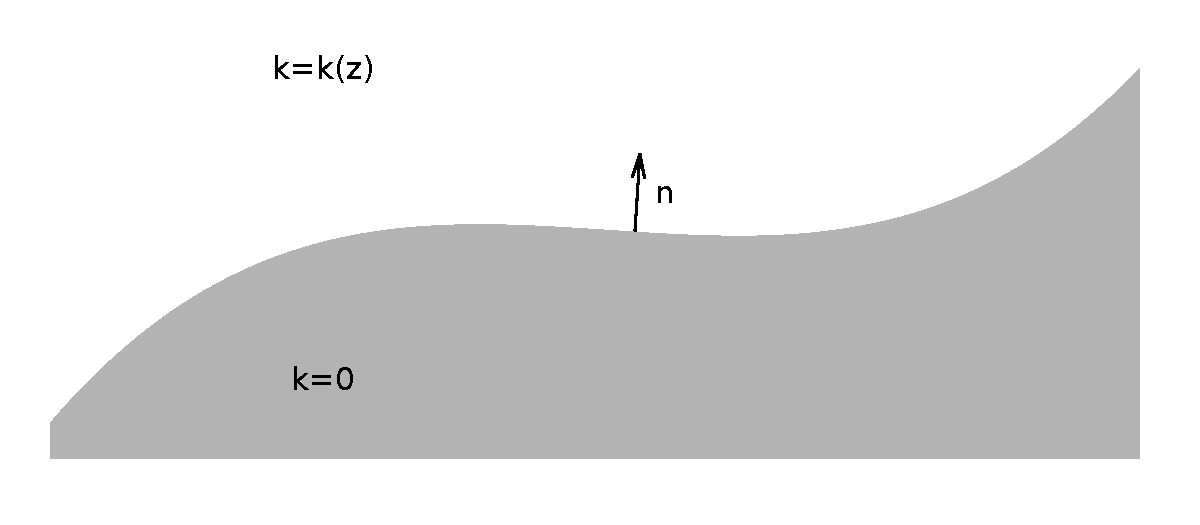
\includegraphics[width=0.75\textwidth]{figs/topography.pdf}
\end{figure*}
Let $S(r)$ is the altitude of the ground surface relative to some reference altitude or depth. In practice it can be relative to the bottom of the comutational domain, or basement, but will be considered sufficiently distant from the bottom that the depth of the basement may be considered infinite. For the wavenumber $k(z)$ we extend 
\begin{equation}
k(z)=\begin{cases}
0 & \text{   if } z<S(r)\\
\frac{\omega^2}{c_{\text{eff}}(z-S(r))^2}+i\alpha_{\text{att}}(z-S(r))+i\alpha_A(z-S(r)) & \text{   if } S(r)<z\\
\end{cases}
\label{eq:k_def_w_basement}\end{equation}
and for the density
\[
\rho(z) =\begin{cases}
\rho_b & \text{   if } z<S(r)\\
\rho_0(z) & \text{   if } S(r)<z.\\
\end{cases}
\]
The ground surface is the locus of points $(r,z)$ satisfying 
\[
z-S(r)=0.
\]
Ground heights specified in the input atmospheric profiles using the Z0 scalar value are used to construct a cubic spline, with repeated endpoints to allow for slight overshoots. This spline returns ground heights interpolated between profiles, as well as their horizonal first and second derivatives.


Eq. \ref{eq:eff_snd_helmholtz} is valid for $z>S(r)$ while for $z<0$
\[
\Big(
\frac{\partial^2}{\partial r^2}+\frac{1}{r}\frac{\partial}{\partial r}
+
\frac{\partial^2}{\partial z^2}
\Big)P(r,z)=0.
\]
These are augmented by the condition that pressure and the normal component of the velocity (or pressure gradient) be continuous at the air/ground interface. Let 
\[
{\bf r}_\pm=\begin{pmatrix}r\\S(r)\\ \end{pmatrix}\pm 0^+ {\bf \hat n}(r)
\]
represent the limiting position on either side of the normal to the gound surface and note that the upward pointing unit normal at a point on the ground surface is given by 
\[
{\bf \hat n}(r)=\begin{pmatrix}n_r(r)\\n_z(r)\\\end{pmatrix}
=\frac{1}{\sqrt{1+S^\prime(r)^2}}\begin{pmatrix}-S^\prime(r)\\ 1\\\end{pmatrix}.
\]
Then
\begin{equation}\label{eq:P_cont_topo}
P({\bf r}_+)=P({\bf r}_-)
\end{equation}
and
\begin{equation}\label{eq:v_cont_topo}
\frac{1}{\rho_0\big(S(r)\big)}{\bf \hat n}(r)\cdot\nabla P|_{{\bf r}_+}
=
\frac{1}{\rho_b}{\bf \hat n}(r)\cdot\nabla P|_{{\bf r}_-}.
\end{equation}
Note that 
\[
{\bf \hat n}(r)\cdot\nabla
=
\frac{1}{\sqrt{1+S^\prime(r)^2}}
\Big(-S^\prime(r)\frac{\partial}{\partial r}+\frac{\partial}{\partial z}\Big).
\]
 
The pressure fields can be scaled as before. For $z>S(r)$ we define 
\[
P(r,z)=\sqrt{\frac{\rho_0(z)}{r}}\tilde P(r,z)=\sqrt{\frac{\rho_0(z)}{r}}e^{ik_0r}p(r,z). 
\]
For $z<S(r)$ the density is constant, so the density scaling doesn't matter, we will do it just to keep the units the same and to make the density gradient zero, setting 
\[
P(r,z)=\sqrt{\frac{\rho_0\big(S(r)\big)}{r}}\tilde P(r,z)=\sqrt{\frac{\rho_0\big(S(r)\big)}{r}}e^{ik_0r}p(r,z). 
\]
Using Eq. \ref{eq:parabolic} one finds 
\[
\frac{\partial p}{\partial r}=ik_0\big(\sqrt{1+Q}-1\big)p
\]
for $z>S(r)$ and 
\[
\frac{\partial p}{\partial r}=ik_0\big(\sqrt{1+Q_0}-1\big)p
\]
for $z<S(r)$
where 
\[
Q_0=\frac{1}{k_0^2}\Big(\frac{d^2}{dz^2}-k_0^2\Big).
\]
The pressure continuity condition, Eq.\ref{eq:P_cont_topo}, becomes 
\[
p({\bf r}_+)=p({\bf r}_-).
\]
Using
\[
\begin{aligned}
\frac{\partial}{\partial r}\sqrt{\frac{1}{r}}\ e^{ik_0r}p(r,z)
&=
\sqrt{\frac{1}{r}}\ e^{ik_0r} \Big(-\frac{1}{2r}+ik_0+\frac{\partial}{\partial r}\Big)p(r,z)\\
&=
\sqrt{\frac{1}{r}}\ e^{ik_0r} \Big(-\frac{1}{2r}+ik_0\sqrt{1+Q}\Big)p(r,z),
\end{aligned}
\]
with $Q$ replaced by $Q_0$ for $z<S(r)$, the condition Eq.\ref{eq:v_cont_topo} becomes 
\begin{equation}
\frac{1}{\rho_0(S(r))}
\Big[ik_0S^\prime(r)\sqrt{1+Q}
-\frac{\partial}{\partial z}-\frac{1}{2}\frac{\rho_0^\prime(z)}{\rho_0(z)}\Big]p\Big|_{{\bf r}_+}
=
\frac{1}{\rho_b}\Big[ik_0S^\prime(r)\sqrt{1+Q_0}-\frac{\partial}{\partial z}
\Big]p\Big|_{{\bf r}_-}
\label{eq:interface_deriv_cond}\end{equation}
where the far field approximation has been used and terms proportional to $\frac{1}{r}$ have been dropped.  

Begin with the case in which the interface is flat. Here $S(r)$ is a constant to be denoted by $z_S$. Let $J$ be the smallest integer with $Jh>z_S$ and we will assume that $J-1<z_S$. Introduce the notation 
\begin{equation}
\begin{aligned}
p_S &=p(r,z_S)\\
J_S &=\frac{z_S}{h}\\
\rho_a &=\rho_0(z_S)\\
\Gamma &=\frac{1}{2}\frac{\rho_0^\prime(z_S)}{\rho_0(z_S)}.
\end{aligned}
\label{eg_flat_gnd_defs}\end{equation} 
We then approximate 
\[
\parderivs{p}{z}\big|_{{\bf r}_+}\approx\frac{p_J-p_S}{(J-J_S)h}
\]
and
\[
\parderivs{p}{z}\big|_{{\bf r}_-}\approx\frac{p_S-p_{J-1}}{(J_S-J+1)h}.
\]
The continuity of $p$ implies that $p_S$ is the pressure at the interface whether measured from above or below. In the case of a flat ground surface $S^\prime(r)=0$ and Eq.\ref{eq:interface_deriv_cond} can be approximated as 
\[
\frac{1}{\rho_a}\Big(\frac{p_J-p_S}{(J-J_S)h}+\Gamma p_S\Big)
\approx
\frac{1}{\rho_b}\frac{p_S-p_{J-1}}{(J_S-J+1)h}.
\]
Solving for $p_S$ one finds 
\[
\begin{aligned}
p_S
&=
\frac{\frac{1}{\rho_b}\frac{p_{J-1}}{J_S-J+1}+\frac{1}{\rho_a}\frac{p_J}{J-J_S}}
{\frac{1}{\rho_b}\frac{1}{J_S-J+1}+\frac{1}{\rho_a}\frac{1}{J-J_S}-h\Gamma}\\
&=
{\cal A}p_J+{\cal B}p_{J-1}, 
\end{aligned}
\]
with
\[
{\cal A}
=
\frac{\frac{1}{\rho_a}\frac{1}{J-J_S}}
{\frac{1}{\rho_b}\frac{1}{J_S-J+1}+\frac{1}{\rho_a}\frac{1}{J-J_S}-h\Gamma}
\]
and
\[
{\cal B}
=
\frac{\frac{1}{\rho_b}\frac{1}{J_S-J+1}}
{\frac{1}{\rho_b}\frac{1}{J_S-J+1}+\frac{1}{\rho_a}\frac{1}{J-J_S}-h\Gamma}.
\]
The finite difference approximation to the second derivatives just above and below the interface are then approximated by
\[
\secparderivs{p}{z}\big|_{{\bf r}_+}
\approx\frac{p_{J+1}-2p_J+p_S}{h^2(J-J_S)}
\approx\frac{p_{J+1}+(-2+{\cal A})p_J+{\cal B}p_{J-1}}{h^2(J-J_S)}
\] 
and 
\[
\secparderivs{p}{z}\big|_{{\bf r}_-}
\approx\frac{p_S-2p_{J-1}+p_{J-2}}{h^2(J_S-J+1)}
\approx\frac{{\cal A}p_J+(-2+{\cal B})p_{J-1}+p_{J-2}}{h^2(J_S-J+1)}.
\]
Note that these forms couple the basement and the atmosphere. 

\begin{equation}\label{eq:Discrete_d^2_flat_interface}
D=
\frac{1}{h^2}\begin{pmatrix}
\ddots&\ddots&\ddots&&&&&&\\
&1&-2&1&&&&&\\
&&1&-2&1&&&&\\
&&&\alpha&\beta&\gamma&&&\\
&&&&a&b&c&&\\
&&&&&1&-2&1&\\
&&&&&&1&-2&1\\
&&&&&&&\ddots&\ddots&\ddots\\
\end{pmatrix}
\end{equation}
where $\beta$ is the $J-1,J-1$ entry and $b$ the $J,J$ entry and 
\[
\begin{aligned}
\alpha &=\frac{1}{J_S-J+1}\\
\beta &=\frac{-2+{\cal B}}{J_S-J+1}\\
\gamma &=\frac{{\cal A}}{J_S-J+1}\\
a &=\frac{{\cal B}}{J-J_S}\\
b &=\frac{-2+{\cal A}}{J-J_S}\\
c &=\frac{1}{J-J_S}\\
\end{aligned}.
\]
Using the specification Eq.\ref{eq:k_def_w_basement} for $k(z)$, the specification Eq.\ref{eq:Q_FD_matrix_def} for the finite difference version of the operator $Q$, which, in this case, includes the interface condition, remains valid. The boundary conditions at the upper and lower limits of the domain have not been specified, but they have no effect. 

As in the flat ground case, we look for a finite difference approximation to the operator $Q$ that includes the interface condition. Assuming such an approximation has been found at a given range $r$, let $J$ be the smallest integer with $Jh>S(r)=z_S$. In addition to the notation introduced in Eq.\ref{eg_flat_gnd_defs}, introduce the notation 
\[
{\bf M}=ik_0S^\prime(r)\sqrt{1+Q}.
\] 
We will see that the resulting expression for ${\bf M}$ changes with each range step. Here we will interprate $Q$ as the finite difference approximation for the current range step. 

As before, approximate 
\[
\parderivs{p}{z}\big|_{{\bf r}_+}\approx\frac{p_J-p_S}{(J-J_S)h},
\]
and, if $(J-1)h\ne S(r)$ (the possibility that $(J-1)h = S(r)$ will have to be considered), 
\[
\parderivs{p}{z}\big|_{{\bf r}_-}\approx\frac{p_S-p_{J-1}}{(J_S-J+1)h}.
\]
As before, the continuity of $p$ implies that $p_S$ is the pressure at the interface whether from above or below. Then Eq.\ref{eq:interface_deriv_cond} becomes 
\[
\frac{1}{\rho_a}\Big(\frac{p_J-p_S}{(J-J_S)h}+\Gamma p_S-({\bf M}p)_J\Big)
\approx
\frac{1}{\rho_b}\Big(\frac{p_S-p_{J-1}}{(J_S-J+1)h}-({\bf M}p)_{J-1}\Big).
\]
Solving for $p_S$ one finds 
\[
\begin{aligned}
p_S
&=
\frac{
	\frac{1}{\rho_b}\frac{p_{J-1}}{J_S-J+1}
	+
	\frac{1}{\rho_a}\frac{p_J}{J-J_S}
	-h\Big(({\bf M}p)_J-({\bf M}p)_{J-1}\Big)
}
{
	\frac{1}{\rho_b}\frac{1}{J_S-J+1}+\frac{1}{\rho_a}\frac{1}{J-J_S}-h\Gamma
}
\\
&={\cal A}p_J+{\cal B}p_{J-1}-\sum_k {\cal M}_{J,k}p_k+\sum_k {\cal M}_{J-1,k}p_k
\end{aligned}
\]
with the matrix ${\cal M}$ defined by 
\[
{\cal M}=
\frac{h}
{
	\frac{1}{\rho_b}\frac{1}{J_S-J+1}+\frac{1}{\rho_a}\frac{1}{J-J_S}-h\Gamma
}
M.
\]
The expression for $p_S$ can now be substituted into the finite difference approximation for $\frac{\partial^2}{\partial z^2}$ giving 
\[
\secparderivs{p}{z}\big|_{{\bf r}_+}
\approx\frac{p_{J+1}+(-2+{\cal A})p_J+{\cal B}p_{J-1}-\sum_k ({\cal M}_{J,k}-{\cal M}_{J-1,k})p_k}{h^2(J-J_S)}
\] 
and 
\[
\secparderivs{p}{z}\big|_{{\bf r}_-}
\approx\frac{{\cal A}p_J+({\cal B}-2)p_{J-1}+p_{J-2}-\sum_k ({\cal M}_{J,k}-{\cal M}_{J-1,k})p_k}{h^2(J_S-J+1)}.
\]
These get substituted into the matrix for $D$. Eq. \ref{eq:Discrete_d^2_flat_interface} remains unchanged except that the vectors
\[
-\frac{1}{h^2(J-J_S)}({\cal M}_{J,k}-{\cal M}_{J-1,k})
\]
and
\[
-\frac{1}{h^2(J_S-J+1)}({\cal M}_{J,k}-{\cal M}_{J-1,k})
\]
get added to the $J^\text{th}$ and $(J-1)^\text{st}$ rows, respectively. 

To proceed further we need an approximation for $\sqrt{1+Q}$. The Taylor expansion gives
\[\begin{aligned}
\sqrt{1+Q}
&=
1+\frac{1}{2}Q-\frac{1}{8}Q^2+\frac{1}{16}Q^3-\frac{5}{128}Q^4
+\cdots+(-1)^n\frac{1\cdot 3\cdot\ldots\cdot (2n-3)}{n!2^n}Q^n+\cdots\\
&= 1+c_1 Q+c_2 Q^2+\dots
\end{aligned}\]
The general $n,m^\text{th}$ order rational approximation is given by 
\[
\sqrt{1+Q}\approx\frac{1+a_1Q+a_2Q^2+\dots+a_nQ^n}{1+b_1Q+b_2Q^2+\dots+b_mQ^m}
\]
An order $1,1$ rational approximation gives
\[
\sqrt{1+Q}\approx\frac{1+\frac{3}{4}Q}{1+\frac{1}{4}Q}
\]
and an order $2,2$ gives 
\[
\sqrt{1+Q}\approx\frac{1+\frac{5}{4}Q+\frac{5}{16}Q^2}{1+\frac{3}{4}Q+\frac{1}{16}Q^2}
\]
\begin{figure*}[h]
  \centering
  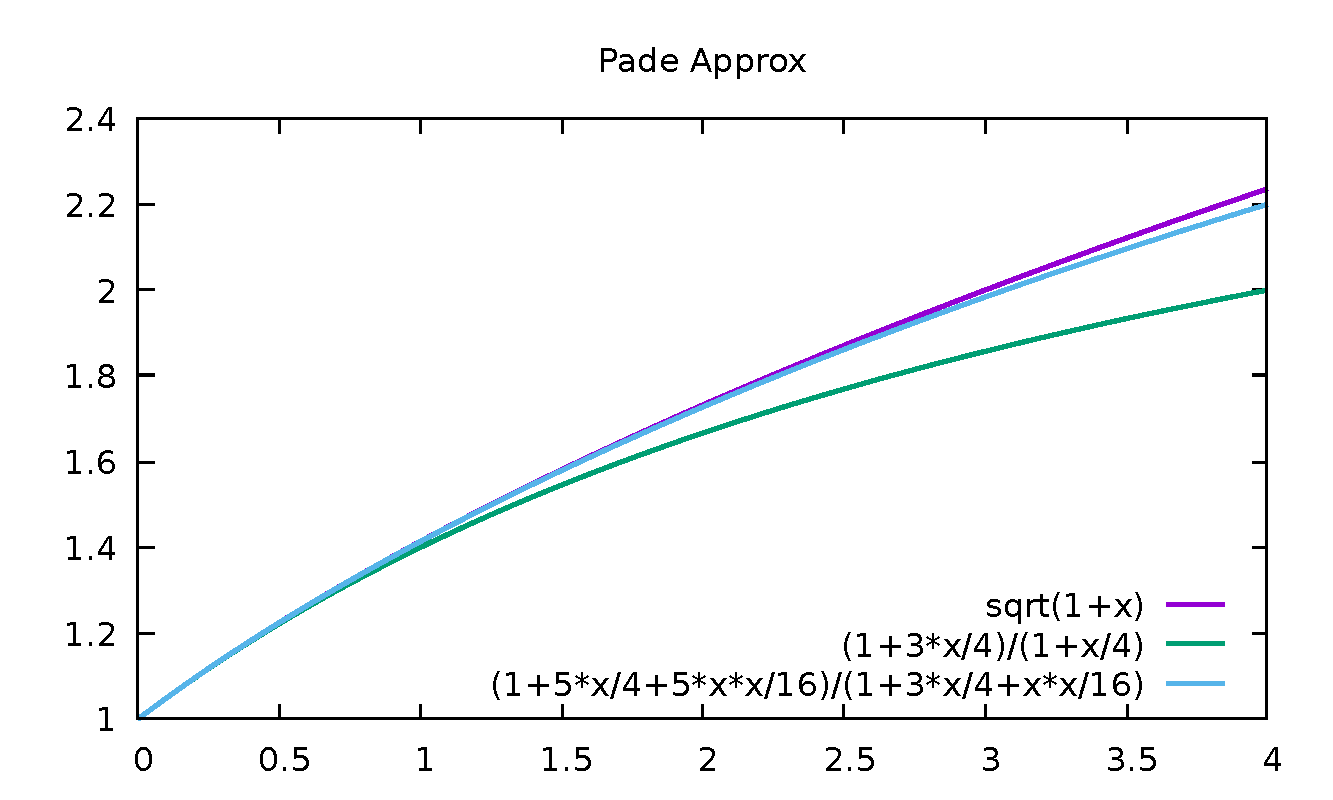
\includegraphics[width=0.45\textwidth]{figs/sqrt_approx.pdf}
  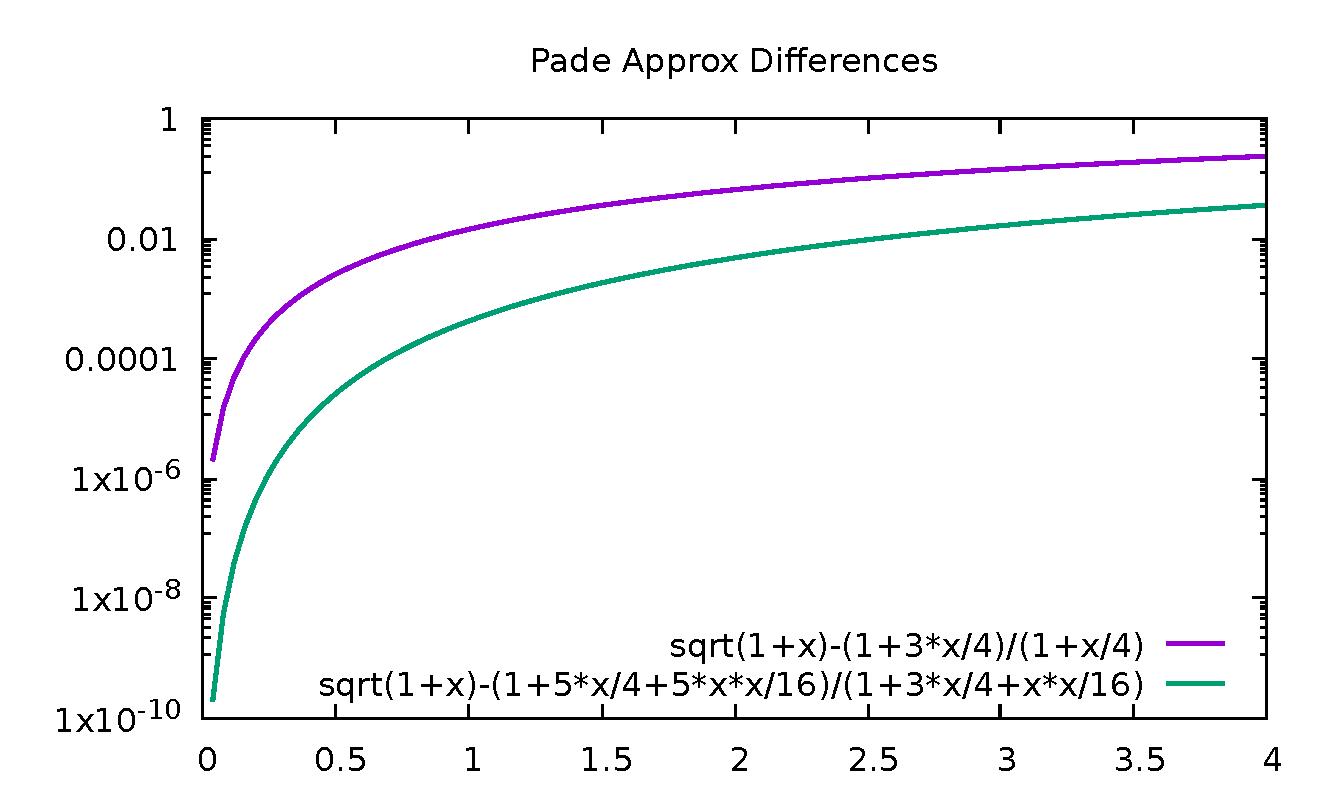
\includegraphics[width=0.45\textwidth]{figs/sqrt_approx_errors.pdf}
\end{figure*} 
These approximations are shown in the figure and can be improved as needed. In the interval $(0,1)$ the order $2,2$ approximation is correct to a part in a thousand. 

To use these rational approximations we need to manage the matrix division. Note that specific rows of ${\bf M}$ are required, in particular the $J^\text{th}$ and $J+1^\text{st}$ rows. In general, if $\mathbf M_K$ is the $K^\text{th}$ row of ${\bf M}$, and if $\mathbf e^{(K)}$ is the vector that is zero except for the $K^\text{th}$ entry, which is 1, then 
\[
\mathbf M_K=\mathbf e^{(K)\, \text{t}}{\bf M}=({\bf M}^\text{t}e^{(K)})^\text{t}. 
\]
Thus, to obtain the $K^\text{th}$ row, one solves the linear system 
\[
\mathbf M_K^\text{t}={\bf M}^\text{t}e^{(K)}. 
\]
This means that all matrix divisions can be implemented using an LU decomposition or similar. For example, the 1,1 rational approximation gives 
\[
(1+\frac{1}{4}Q^\text{t})\mathbf M_K^\text{t}=(1+\frac{3}{4}Q^\text{t})e^{(K)}.
\]
Currently, the 3,4 approximation is being used throughout. 


\subsection{Running ePape}
\label{sec: running ePape}

Making sure that the executable for {\bf ePape} is in the system's path, it can be run by entering 
\begin{verbatim} 
    ePape [--option1 val1] [--option2 val2] [...] [--flag1] [...] 
\end{verbatim}
on a command line. Generally, options are followed by values, either numbers, strings or filenames. Flags are not. 
Entering \verb"ePape --help" sends the following help page to the screen:

\begin{verbatim}
By default the program computes both the 1D (at the ground) and 2D transfer
function and saves the data to 2 files:
    file tloss_1d.pe - transfer function at the ground
    file tloss_2d.pe - full 2-D transfer function field

The options below can be specified in a colon-separated file "epade_pe.param" or
at the command line. Command-line options override file options.

Options Control:
  --help                 Prints help test
  --paramfile            Parameter file name [epade_pe.param]
  --printparams          Print parameter summary to screen

Atmosphere:
  --atmosfile            1-D atmospheric profile filename
  --atmosfile2d          2-D atmospheric summary filename (see manual)

Required Parameters:
  --freq                 Frequency of analysis (Hz)
  --starter              Starter type: one of { self, gaussian, user }
  --maxrange_km          Maximum range in km to use for modeling

Modes of Operation:
  --singleprop           Single azimuth propagation. Requires --azimuth
    --azimuth            Propagation azimuth ( degrees clockwise from north,
                         [0,360) )
  --multiprop            Multiple azimuth propagation. Requires --azimuth_start,
                         --azimuth_end, and --azimuth_step, disables
                         --atmosfile2d
    --azimuth_start      Starting azimuth, in degrees CW from North [0,360)
    --azimuth_end        Ending azimuth, in degrees CW from North [0,360)
    --azimuth_step       Azimuth step, in degrees CW from North [0,360)

Optional Parameters [default]:
  --atmosheaderfile      External header file, overrides internal header [None]
  --npade                Number of Pade coefficients to use [4]
  --dz_m                 Altitude resolution in meters [automatic]
  --maxheight_km         Maximum height of analysis in km [150.0, or max height
                         of atmosphere]
  --sourceheight_km      Source height in km [ground]
  --receiverheight_km    Receiver height in km [ground]
  --groundheight_km      Ground height in km [Z0 parameter in profile, or 0.0]
  --Nrng_steps           Number of range steps to use [decide internally]
  --ground_impedence_real
                         Real part of ground impedence [rigid ground]
  --ground_impedence_imag
                         Imaginary part of ground impedence [rigid ground]
  --starterfile          File name containing starter [n/a]. Columns are
                         Height(km) RealPart ImaginaryPart
  --attnfile             File name containing attenuation, to override default
                         Sutherland/Bass [n/a]. Columns are
                         Height(km) Attenuation(np/m)

Flags:
  --write_2d_tloss       Output 2-D transfer function to tloss_2d.pe
  --write_atm_profile    Output atmospheric profile to atm_profile.pe
  --write_starter        Output starter to starter.pe
  --write_topography     Output interpolated topography to topography.pe
  --lossless             Ignore atmospheric attenuation
  --topo                 Use topography. Requires presence of 'Z0' parameter in
                         atmospheric files



OUTPUT Files: Format description (column order):
  tloss_1d.pe:                 r (km), az (deg), TF (real), TF (imag)
  tloss_multiplot.pe           r (km), az (deg), TF (real), TF (imag)
  tloss_2d.pe:                 r, z, TF (real), TF (imag)
  atm_profile.pe:              z,u,v,w,t,d,p,c,c_eff
  starter.pe:                  z, starter (real), starter(imag)
  topography.pe:               az, r, z0

Examples (run from 'samples' directory):

    ../bin/ePape --singleprop --starter self --atmosfile \
         NCPA_canonical_profile_trimmed.dat --freq 0.1 --azimuth 90 \
         --maxrange_km 1000

    ../bin/ePape --singleprop --starter self --atmosfile2d \
         toy_profile_2d_summary.dat --freq 0.5 --azimuth 90 --maxrange_km 1800 \
         --write_2d_tloss

    ../bin/ePape --multiprop --starter self --atmosfile \
         NCPA_canonical_profile_trimmed.dat --freq 0.5 --azimuth_start 0 \
         --azimuth_end 360 --azimuth_step 2 --maxrange_km 1000

    ../bin/ePape --singleprop --topo --starter self --atmosfile2d \
         toy_profile_2d_summary_topo.dat --freq 0.5 --azimuth 90 --maxrange_km \
         1200 --write_2d_tloss --write_topography

\end{verbatim}

The basic functionality of ePape is to produce a single frequency transfer function for signal propagation in the effective sound speed approximation. Explicitly, the long range propagated acoustic pressure amplitude at a single frequency produced by a unit point source at a reference range of 1 km is computed. The density scaled pressure, $\rho_0^{-\frac{1}{2}}P$, is written to files. The magnitude of the transfer function is referred to as the signal attenuation. To obtain the physical attenuation the output must be multiplied by $\rho_0^{-\frac{1}{2}}$; however, for purposes of visualization this is not advised since the physical acoustic pressure decreases dramatically with increasing altitude, making it difficult to visualize. The attenuation in dB relative to 1 is referred to as the transmission loss.

\verb+Options Control:+ Parameters and options can be sent to {\bf ePape} either on the command line, or through a parameter file \verb+epade_pe.param+ by setting the option \verb+--paramfile+. The option \verb+--printparams+ causes the current parameter set to be printed to the screen.

\verb+Atmosphere:+ The input of atmospheric profiles is currently through ascii files specified using \verb+--atmosfile+ or \verb+--atmosfile2d+. The \verb+--atmosfile+ flag indicates that a stratified model atmosphere is being used, and a single file is specified. The \verb+--atmosfile2d+ flag indicates that a range dependent model atmosphere is being used and is specified through an atmospheric summary file. The summary file has two columns, range and filename; the files contain the atmospheric specifications valid at the indicated range. Binary format input is under development.
 
\verb+Modes of Operation:+ Using the \verb+--singleprop+ option the attenuation along a single azimuth is computed. By default, the attenuation along the ground is saved in \verb+tloss_1d.pe+ and the attenuation in the entire range/altitude plane is saved in \verb+tloss_2d.pe+. With the \verb+--multiprop+ option the attenuation along a specified grid of azimuths is computed and stored in \verb+tloss_multiplot.pe+. In \verb+tloss_multiplot.pe+ data is stored in line seperated blocks of constant range. \verb+--multiprop+ uses the functionality of \verb+--singleprop+ for each azimuth. For convenience, the column format in \verb+tloss_1d.pe+ is the same as \verb+tloss_multiplot.pe+ in that the azimuth is saved in the second column. Currently, only stratified atmospheres are supported for \verb+--multiprop+. Support for range dependent atmospheres is under development. The \verb+--topo+ option causes {\bf ePape} to introduce the high density basement with interface given by a cubic spline of from the \verb+Z0+ values in the atmospheric profile files. Note that \verb+--topo+ is intrinsically range dependent and requires a summary file referencing a directory of profile files. The flag \verb+--write_topography+ causes the interpolated ground elevation to be written to a file. 

\verb+Optional Parameters:+ Parameters can be changed from their default values. The \verb+--npade+ flag allows the user to choose the degree of the polynomial in the denomenator of the Pad\'e approximant. The default is 4. Note that the numerator has degree one less than the denominator. The \verb+dz_m+ flag allows the user to choose the altitude resolution. The default is the closest value to 20 points per wavelength, computed on the ground, that respects a uniform grid. The user has control over the numnber of range steps through \verb+--Nrng_steps+. The default range step is one wavelength, estimated using the nomunal sound speed 340 m/s. A ground impedence value can be input using the \verb+--ground_impedence_real+ and \verb+--ground_impedence_imag+ flags. 


\subsection{Running ePape: examples}
\label{sec: pade examples}

The {\bf ePape} help page ends with three examples designed to be run in the \verb+samples+ directory. 

\noindent 1) The first example is propagation a the stratified model atmosphere, the NCPA toy atmosphere, with source on the ground. The command line is 
\begin{verbatim}
    ../bin/ePape --singleprop --starter self --atmosfile \
         NCPA_canonical_profile_trimmed.dat --freq 0.1 --azimuth 90 \
         --maxrange_km 1000
\end{verbatim}
and the results are shown in Fig.\,\ref{fig: ePape ex1}. The 1d transmission loss for ground to ground propagation is shown on the left plotted as transmission loss versus range, and the 2d transmission loss in the full range-altitude plane is shown on the right plotted as altitude versus range with transmission loss indicated by color. 

\begin{figure}[h]
\begin{center}
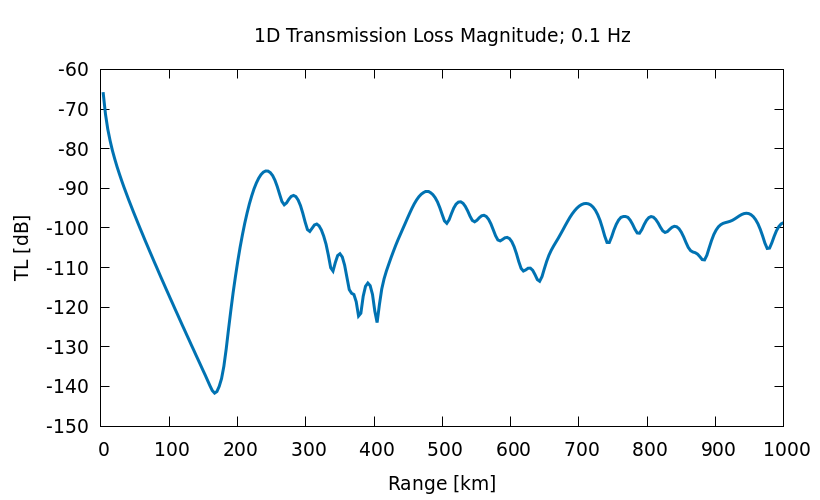
\includegraphics[width=0.49\textwidth]{figs/ePape_ex1_1d}
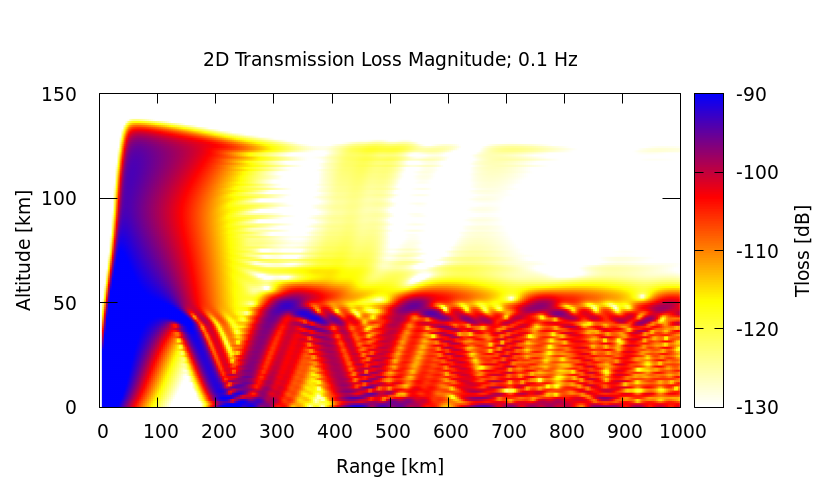
\includegraphics[width=0.49\textwidth]{figs/ePape_ex1_2d}
\end{center}
\caption{1D and 2D transmission loss magnitudes at 0.1 Hz obtained with {\bf ePape} for eastward ground-to-ground propagation in the NCPA toy atmosphere shown in Figure \ref{fig:canonic_sound_speeds}. Shown is the lossy transmission loss magnitude. The 1D transmission loss is shown in the left panel and the 2D transmission loss is shown in the right panel.}
\label{fig: ePape ex1}
\end{figure}

\noindent 2) The second example shows how to input a range dependent atmosphere. The command line is 
\begin{verbatim}
    ../bin/ePape --singleprop --starter self --atmosfile2d \
         toy_profile_2d_summary.dat --freq 0.5 --azimuth 90 --maxrange_km 1800 \
         --write_2d_tloss
\end{verbatim}
The contents of the summary file \verb+toy_profile_2d_summary.dat+ are shown below. 
\begin{verbatim}
0.0   toy_profiles/toy_soundspeed_jetstr0.dat
350.0  toy_profiles/toy_soundspeed_jetstr2.dat
500.0  toy_profiles/toy_soundspeed_jetstr4.dat
650.0  toy_profiles/toy_soundspeed_jetstr6.dat
800.0  toy_profiles/toy_soundspeed_jetstr8.dat
\end{verbatim}
Each row contains a range (in km) and a file name. The range indicates where the model atmosphere given in the corresponding file is to commence. In this example, propagation is directly to the east. The model zonal winds and the corresponding effective sound speeds are shown in Fig.\,\ref{fig: ePape ex2 profiles}. In Fig.\,\ref{fig: ePape ex2} the 1d transmission loss for ground to ground propagation is shown on the left plotted as transmission loss versus range, and the 2d transmission loss in the full range-altitude plane is shown on the right plotted as altitude versus range with transmission loss indicated by color. 

\begin{figure}[h]
\begin{center}
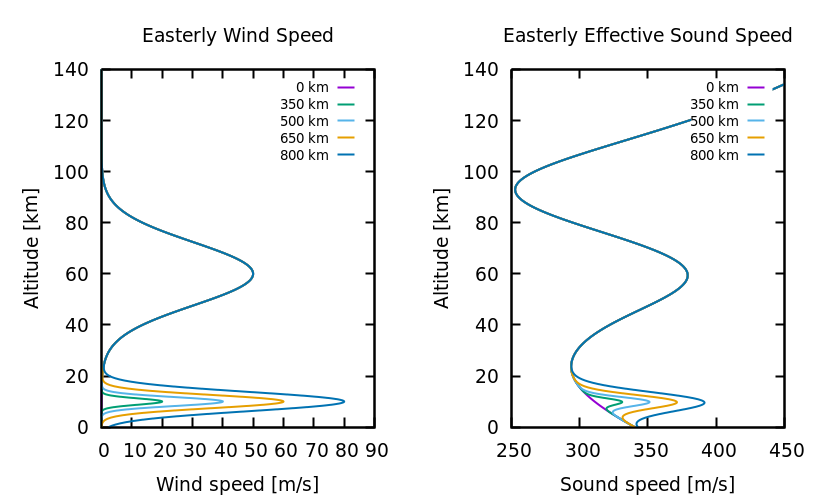
\includegraphics[width=0.5\textwidth]{figs/ePape_ex2_profiles.png}
\end{center}
\caption{The zonal winds and associated effective sound speed profiles from the example range dependent atmosphere used in example 2.}
\label{fig: ePape ex2 profiles}
\end{figure}


\begin{figure}[h]
\begin{center}
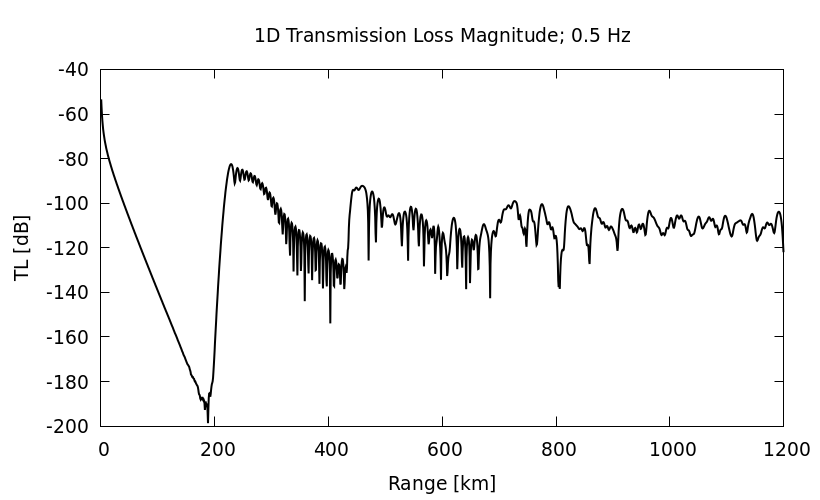
\includegraphics[width=0.49\textwidth]{figs/ePape_ex2_1d}
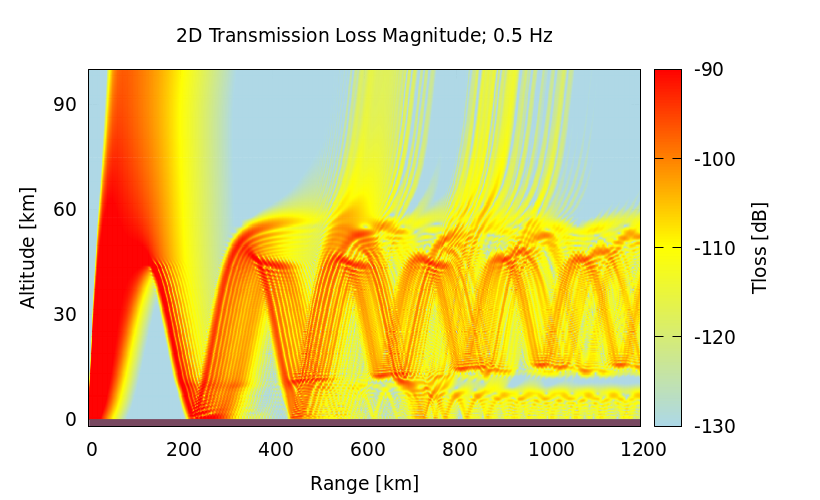
\includegraphics[width=0.49\textwidth]{figs/ePape_ex2_2d}
\end{center}
\caption{1D and 2D transmission loss magnitudes at 0.5 Hz obtained with {\bf ePape} for eastward ground-to-ground propagation in the range dependent atmosphere specified by the summary file {\tt toy\_profile\_2d\_summary.dat}. Shown is the lossy transmission loss magnitude. The 1d transmission loss on the left and the 2d on the right.}
\label{fig: ePape ex2}
\end{figure}

\noindent 3) The third example shows how to use the \verb+--multiplot+ option for the NCPA toy atmosphere. The command line is
\begin{verbatim}
    ../bin/ePape --multiprop --starter self --atmosfile \
         NCPA_canonical_profile_trimmed.dat --freq 0.5 --azimuth_start 0 \
         --azimuth_end 360 --azimuth_step 2 --maxrange_km 1000
\end{verbatim}
The lossless and lossy results are shown in Fig.\,\ref{fig: ePape ex3}. 
         
\begin{figure}[h]
\begin{center}
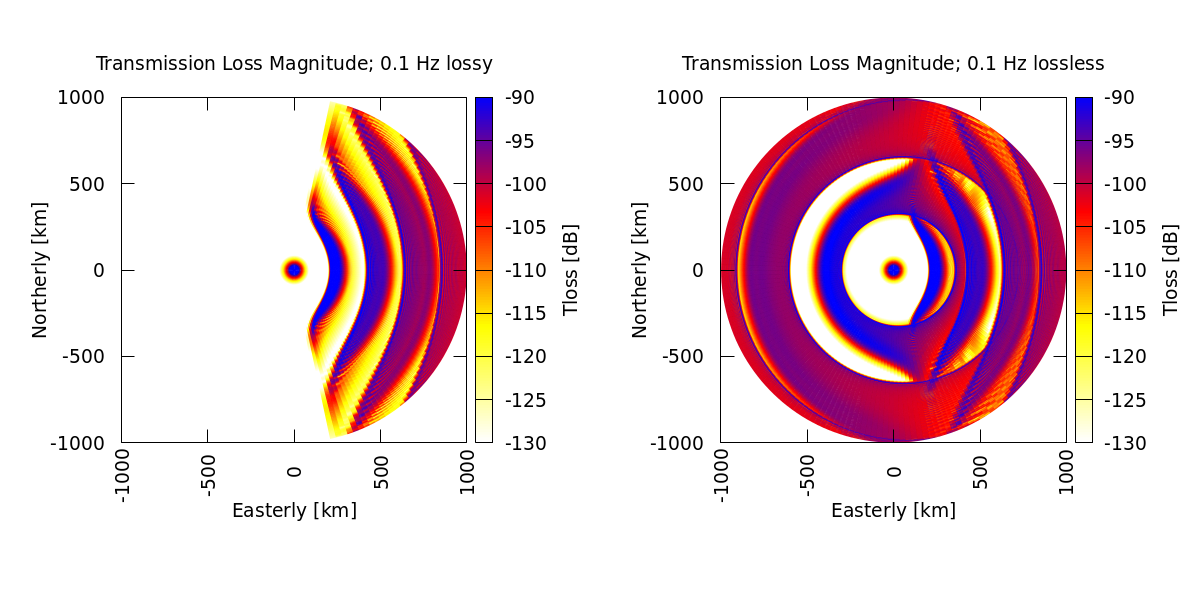
\includegraphics[width=0.9\textwidth]{figs/ePape_ex3}
\end{center}
\caption{Multiplot option output. Shown on the left is the lossy transmission loss magnitude and on the right the lossless transmission loss magnitude.}
\label{fig: ePape ex3}
\end{figure}

\noindent 4) The fourth example shows how to use the \verb+--topo+ option(s). Usage is similar to the use of {\bf ePape} with range dependence. The command line is 
\begin{verbatim}
    ../bin/ePape --singleprop --topo --starter self --atmosfile2d \
         toy_profile_2d_summary_topo.dat --freq 0.5 --azimuth 90 --maxrange_km \
         1200 --write_2d_tloss --write_topography
\end{verbatim}
The profiles are the same as in \ref{fig: ePape ex2 profiles} of example 2, except that there are non-zero values of \verb+Z0+ in some of the profile file headers. 
\begin{figure}[h]
\begin{center}
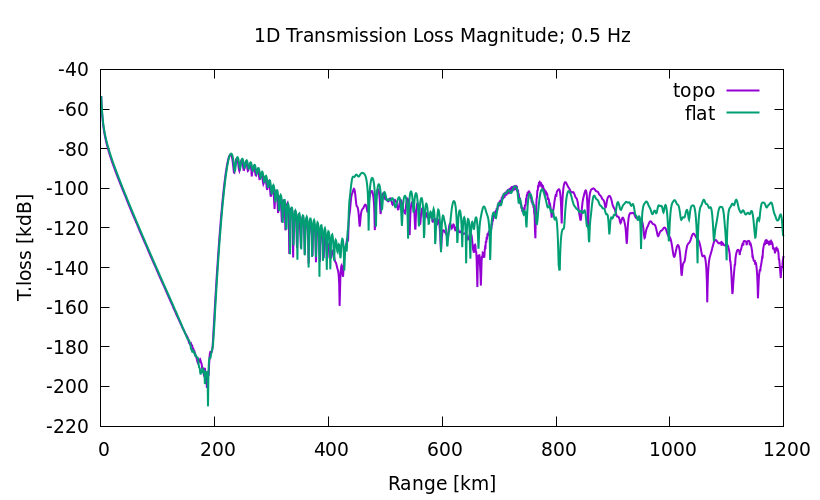
\includegraphics[width=0.49\textwidth]{figs/ePape_ex4_1d}
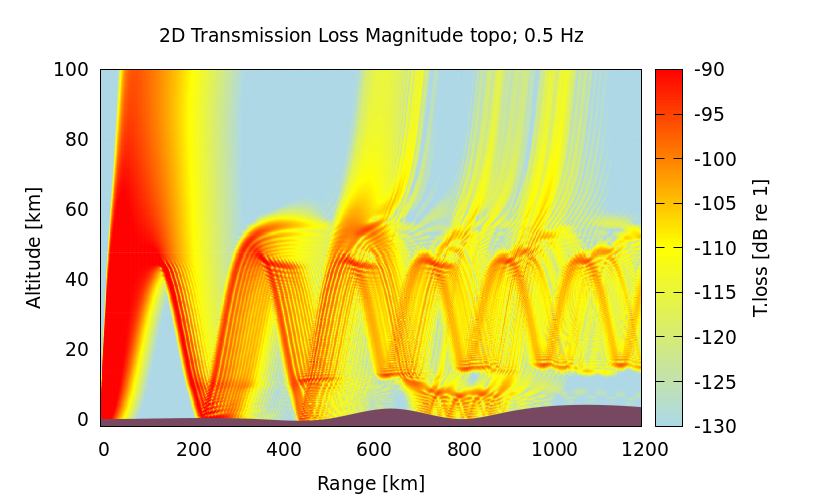
\includegraphics[width=0.49\textwidth]{figs/ePape_ex4_2d}
\end{center}
\caption{Topo option output for the atmosphere of example 2. Shown on the left is a comparison between ground-to-ground 1d transmission loss magnitudes over flat ground and over undulating ground. On the right is the 2d transmission loss magnitude over undulating ground. The topography is mapped out in the 2d plot.}
\label{fig: ePape ex4}
\end{figure}

